\documentclass[1p]{elsarticle_modified}
%\bibliographystyle{elsarticle-num}

%\usepackage[colorlinks]{hyperref}
%\usepackage{abbrmath_seonhwa} %\Abb, \Ascr, \Acal ,\Abf, \Afrak
\usepackage{amsfonts}
\usepackage{amssymb}
\usepackage{amsmath}
\usepackage{amsthm}
\usepackage{scalefnt}
\usepackage{amsbsy}
\usepackage{kotex}
\usepackage{caption}
\usepackage{subfig}
\usepackage{color}
\usepackage{graphicx}
\usepackage{xcolor} %% white, black, red, green, blue, cyan, magenta, yellow
\usepackage{float}
\usepackage{setspace}
\usepackage{hyperref}

\usepackage{tikz}
\usetikzlibrary{arrows}

\usepackage{multirow}
\usepackage{array} % fixed length table
\usepackage{hhline}

%%%%%%%%%%%%%%%%%%%%%
\makeatletter
\renewcommand*\env@matrix[1][\arraystretch]{%
	\edef\arraystretch{#1}%
	\hskip -\arraycolsep
	\let\@ifnextchar\new@ifnextchar
	\array{*\c@MaxMatrixCols c}}
\makeatother %https://tex.stackexchange.com/questions/14071/how-can-i-increase-the-line-spacing-in-a-matrix
%%%%%%%%%%%%%%%

\usepackage[normalem]{ulem}

\newcommand{\msout}[1]{\ifmmode\text{\sout{\ensuremath{#1}}}\else\sout{#1}\fi}
%SOURCE: \msout is \stkout macro in https://tex.stackexchange.com/questions/20609/strikeout-in-math-mode

\newcommand{\cancel}[1]{
	\ifmmode
	{\color{red}\msout{#1}}
	\else
	{\color{red}\sout{#1}}
	\fi
}

\newcommand{\add}[1]{
	{\color{blue}\uwave{#1}}
}

\newcommand{\replace}[2]{
	\ifmmode
	{\color{red}\msout{#1}}{\color{blue}\uwave{#2}}
	\else
	{\color{red}\sout{#1}}{\color{blue}\uwave{#2}}
	\fi
}

\newcommand{\Sol}{\mathcal{S}} %segment
\newcommand{\D}{D} %diagram
\newcommand{\A}{\mathcal{A}} %arc


%%%%%%%%%%%%%%%%%%%%%%%%%%%%%5 test

\def\sl{\operatorname{\textup{SL}}(2,\Cbb)}
\def\psl{\operatorname{\textup{PSL}}(2,\Cbb)}
\def\quan{\mkern 1mu \triangleright \mkern 1mu}

\theoremstyle{definition}
\newtheorem{thm}{Theorem}[section]
\newtheorem{prop}[thm]{Proposition}
\newtheorem{lem}[thm]{Lemma}
\newtheorem{ques}[thm]{Question}
\newtheorem{cor}[thm]{Corollary}
\newtheorem{defn}[thm]{Definition}
\newtheorem{exam}[thm]{Example}
\newtheorem{rmk}[thm]{Remark}
\newtheorem{alg}[thm]{Algorithm}

\newcommand{\I}{\sqrt{-1}}
\begin{document}

%\begin{frontmatter}
%
%\title{Boundary parabolic representations of knots up to 8 crossings}
%
%%% Group authors per affiliation:
%\author{Yunhi Cho} 
%\address{Department of Mathematics, University of Seoul, Seoul, Korea}
%\ead{yhcho@uos.ac.kr}
%
%
%\author{Seonhwa Kim} %\fnref{s_kim}}
%\address{Center for Geometry and Physics, Institute for Basic Science, Pohang, 37673, Korea}
%\ead{ryeona17@ibs.re.kr}
%
%\author{Hyuk Kim}
%\address{Department of Mathematical Sciences, Seoul National University, Seoul 08826, Korea}
%\ead{hyukkim@snu.ac.kr}
%
%\author{Seokbeom Yoon}
%\address{Department of Mathematical Sciences, Seoul National University, Seoul, 08826,  Korea}
%\ead{sbyoon15@snu.ac.kr}
%
%\begin{abstract}
%We find all boundary parabolic representation of knots up to 8 crossings.
%
%\end{abstract}
%\begin{keyword}
%    \MSC[2010] 57M25 
%\end{keyword}
%
%\end{frontmatter}

%\linenumbers
%\tableofcontents
%
\newcommand\colored[1]{\textcolor{white}{\rule[-0.35ex]{0.8em}{1.4ex}}\kern-0.8em\color{red} #1}%
%\newcommand\colored[1]{\textcolor{white}{ #1}\kern-2.17ex	\textcolor{white}{ #1}\kern-1.81ex	\textcolor{white}{ #1}\kern-2.15ex\color{red}#1	}

{\Large $\underline{11a_{266}~(K11a_{266})}$}

\setlength{\tabcolsep}{10pt}
\renewcommand{\arraystretch}{1.6}
\vspace{1cm}\begin{tabular}{m{100pt}>{\centering\arraybackslash}m{274pt}}
\multirow{5}{120pt}{
	\centering
	\includegraphics[width=112pt]{../../../GIT/diagram.site/Diagrams/png/515_11a_266.png}\\
\ \ \ A knot diagram\footnotemark}&
\allowdisplaybreaks
\textbf{Linearized knot diagam} \\
\cline{2-2}
 &
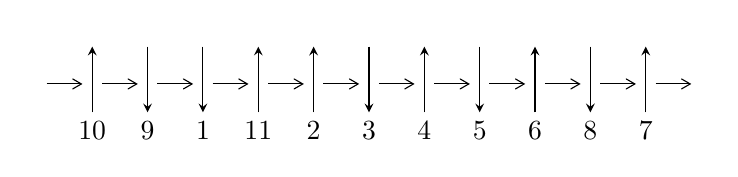
\begin{tikzpicture}[x=20pt, y=17pt]
	% nodes
	\node (C0) at (0, 0) {};
	\node (C1) at (1, 0) {};
	\node (C1U) at (1, +1) {};
	\node (C1D) at (1, -1) {10};

	\node (C2) at (2, 0) {};
	\node (C2U) at (2, +1) {};
	\node (C2D) at (2, -1) {9};

	\node (C3) at (3, 0) {};
	\node (C3U) at (3, +1) {};
	\node (C3D) at (3, -1) {1};

	\node (C4) at (4, 0) {};
	\node (C4U) at (4, +1) {};
	\node (C4D) at (4, -1) {11};

	\node (C5) at (5, 0) {};
	\node (C5U) at (5, +1) {};
	\node (C5D) at (5, -1) {2};

	\node (C6) at (6, 0) {};
	\node (C6U) at (6, +1) {};
	\node (C6D) at (6, -1) {3};

	\node (C7) at (7, 0) {};
	\node (C7U) at (7, +1) {};
	\node (C7D) at (7, -1) {4};

	\node (C8) at (8, 0) {};
	\node (C8U) at (8, +1) {};
	\node (C8D) at (8, -1) {5};

	\node (C9) at (9, 0) {};
	\node (C9U) at (9, +1) {};
	\node (C9D) at (9, -1) {6};

	\node (C10) at (10, 0) {};
	\node (C10U) at (10, +1) {};
	\node (C10D) at (10, -1) {8};

	\node (C11) at (11, 0) {};
	\node (C11U) at (11, +1) {};
	\node (C11D) at (11, -1) {7};
	\node (C12) at (12, 0) {};

	% arrows
	\draw[->,>={angle 60}]
	(C0) edge (C1) (C1) edge (C2) (C2) edge (C3) (C3) edge (C4) (C4) edge (C5) (C5) edge (C6) (C6) edge (C7) (C7) edge (C8) (C8) edge (C9) (C9) edge (C10) (C10) edge (C11) (C11) edge (C12) ;	\draw[->,>=stealth]
	(C1D) edge (C1U) (C2U) edge (C2D) (C3U) edge (C3D) (C4D) edge (C4U) (C5D) edge (C5U) (C6U) edge (C6D) (C7D) edge (C7U) (C8U) edge (C8D) (C9D) edge (C9U) (C10U) edge (C10D) (C11D) edge (C11U) ;
	\end{tikzpicture} \\
\hhline{~~} \\& 
\textbf{Solving Sequence} \\ \cline{2-2} 
 &
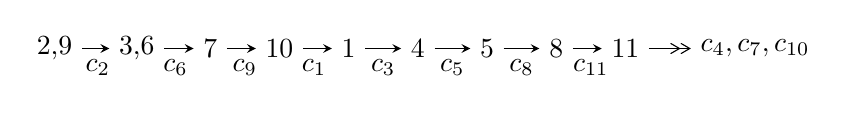
\begin{tikzpicture}[x=25pt, y=7pt]
	% node
	\node (A0) at (-1/8, 0) {2,9};
	\node (A1) at (17/16, 0) {3,6};
	\node (A2) at (17/8, 0) {7};
	\node (A3) at (25/8, 0) {10};
	\node (A4) at (33/8, 0) {1};
	\node (A5) at (41/8, 0) {4};
	\node (A6) at (49/8, 0) {5};
	\node (A7) at (57/8, 0) {8};
	\node (A8) at (65/8, 0) {11};
	\node (C1) at (1/2, -1) {$c_{2}$};
	\node (C2) at (13/8, -1) {$c_{6}$};
	\node (C3) at (21/8, -1) {$c_{9}$};
	\node (C4) at (29/8, -1) {$c_{1}$};
	\node (C5) at (37/8, -1) {$c_{3}$};
	\node (C6) at (45/8, -1) {$c_{5}$};
	\node (C7) at (53/8, -1) {$c_{8}$};
	\node (C8) at (61/8, -1) {$c_{11}$};
	\node (A9) at (10, 0) {$c_{4},c_{7},c_{10}$};

	% edge
	\draw[->,>=stealth]	
	(A0) edge (A1) (A1) edge (A2) (A2) edge (A3) (A3) edge (A4) (A4) edge (A5) (A5) edge (A6) (A6) edge (A7) (A7) edge (A8) ;
	\draw[->>,>={angle 60}]	
	(A8) edge (A9);
\end{tikzpicture} \\ 

\end{tabular} \\

\footnotetext{
The image of knot diagram is generated by the software ``\textbf{Draw programme}" developed by Andrew Bartholomew(\url{http://www.layer8.co.uk/maths/draw/index.htm\#Running-draw}), where we modified some parts for our purpose(\url{https://github.com/CATsTAILs/LinksPainter}).
}\phantom \\ \newline 
\centering \textbf{Ideals for irreducible components\footnotemark of $X_{\text{par}}$} 
 
\begin{align*}
I^u_{1}&=\langle 
2.09838\times10^{20} u^{29}+6.55534\times10^{21} u^{28}+\cdots+1.72668\times10^{21} b+1.91679\times10^{23},\\
\phantom{I^u_{1}}&\phantom{= \langle  }7.48748\times10^{20} u^{29}+2.12940\times10^{22} u^{28}+\cdots+3.45337\times10^{21} a+2.83237\times10^{23},\\
\phantom{I^u_{1}}&\phantom{= \langle  }u^{30}+29 u^{29}+\cdots+5632 u+512\rangle \\
I^u_{2}&=\langle 
222790111 u^{46}-4153864769 u^{45}+\cdots+2281728 b+6714872532,\\
\phantom{I^u_{2}}&\phantom{= \langle  }-2238290844 u^{46} a-21314380402 u^{46}+\cdots-16228635188 a-83493140173,\\
\phantom{I^u_{2}}&\phantom{= \langle  }u^{47}-14 u^{46}+\cdots+30 u-3\rangle \\
I^u_{3}&=\langle 
-1345 u^{15}+7729 u^{14}+\cdots+3655 b+38,\;-38 u^{15}-1117 u^{14}+\cdots+3655 a+12877,\\
\phantom{I^u_{3}}&\phantom{= \langle  }u^{16}-6 u^{15}+\cdots+u+1\rangle \\
I^u_{4}&=\langle 
3 a u+3 b+2 u+3,\;3 a^2- a u- a+1,\;u^2+3 u+3\rangle \\
\\
\end{align*}
\raggedright * 4 irreducible components of $\dim_{\mathbb{C}}=0$, with total 144 representations.\\
\footnotetext{All coefficients of polynomials are rational numbers. But the coefficients are sometimes approximated in decimal forms when there is not enough margin.}
\newpage
\renewcommand{\arraystretch}{1}
\centering \section*{I. $I^u_{1}= \langle 2.10\times10^{20} u^{29}+6.56\times10^{21} u^{28}+\cdots+1.73\times10^{21} b+1.92\times10^{23},\;7.49\times10^{20} u^{29}+2.13\times10^{22} u^{28}+\cdots+3.45\times10^{21} a+2.83\times10^{23},\;u^{30}+29 u^{29}+\cdots+5632 u+512 \rangle$}
\flushleft \textbf{(i) Arc colorings}\\
\begin{tabular}{m{7pt} m{180pt} m{7pt} m{180pt} }
\flushright $a_{2}=$&$\begin{pmatrix}1\\0\end{pmatrix}$ \\
\flushright $a_{9}=$&$\begin{pmatrix}0\\u\end{pmatrix}$ \\
\flushright $a_{3}=$&$\begin{pmatrix}1\\u^2\end{pmatrix}$ \\
\flushright $a_{6}=$&$\begin{pmatrix}-0.216817 u^{29}-6.16616 u^{28}+\cdots-843.133 u-82.0175\\-0.121527 u^{29}-3.79649 u^{28}+\cdots-1139.09 u-111.010\end{pmatrix}$ \\
\flushright $a_{7}=$&$\begin{pmatrix}0.176923 u^{29}+4.51009 u^{28}+\cdots-277.468 u-33.2290\\0.726411 u^{29}+20.5852 u^{28}+\cdots+2839.46 u+269.003\end{pmatrix}$ \\
\flushright $a_{10}=$&$\begin{pmatrix}0.0737630 u^{29}+2.11244 u^{28}+\cdots+454.512 u+44.0773\\0.0266890 u^{29}+0.858935 u^{28}+\cdots+372.356 u+37.7667\end{pmatrix}$ \\
\flushright $a_{1}=$&$\begin{pmatrix}-0.181935 u^{29}-4.87001 u^{28}+\cdots-131.180 u-9.97749\\-0.321147 u^{29}-9.00243 u^{28}+\cdots-1126.22 u-106.815\end{pmatrix}$ \\
\flushright $a_{4}=$&$\begin{pmatrix}-0.344913 u^{29}-9.38133 u^{28}+\cdots-491.954 u-39.3302\\-0.241720 u^{29}-7.27828 u^{28}+\cdots-1882.54 u-183.233\end{pmatrix}$ \\
\flushright $a_{5}=$&$\begin{pmatrix}-0.0952900 u^{29}-2.36967 u^{28}+\cdots+295.961 u+28.9927\\-0.121527 u^{29}-3.79649 u^{28}+\cdots-1139.09 u-111.010\end{pmatrix}$ \\
\flushright $a_{8}=$&$\begin{pmatrix}-0.0645692 u^{29}-1.79489 u^{28}+\cdots-175.655 u-17.7913\\0.111643 u^{29}+3.04839 u^{28}+\cdots+259.810 u+24.1019\end{pmatrix}$ \\
\flushright $a_{11}=$&$\begin{pmatrix}-0.293270 u^{29}-8.33770 u^{28}+\cdots-1123.71 u-104.995\\0.527885 u^{29}+14.3259 u^{28}+\cdots+755.639 u+64.5890\end{pmatrix}$\\ \flushright $a_{11}=$&$\begin{pmatrix}-0.293270 u^{29}-8.33770 u^{28}+\cdots-1123.71 u-104.995\\0.527885 u^{29}+14.3259 u^{28}+\cdots+755.639 u+64.5890\end{pmatrix}$\\&\end{tabular}
\flushleft \textbf{(ii) Obstruction class $= -1$}\\~\\
\flushleft \textbf{(iii) Cusp Shapes $= \frac{190232019886448235663}{431670906353547523808} u^{29}+\frac{1299412671514678966295}{107917726588386880952} u^{28}+\cdots+\frac{3145923075548619685658}{13489715823548360119} u+\frac{100943563341881674894}{13489715823548360119}$}\\~\\
\newpage\renewcommand{\arraystretch}{1}
\flushleft \textbf{(iv) u-Polynomials at the component}\newline \\
\begin{tabular}{m{50pt}|m{274pt}}
Crossings & \hspace{64pt}u-Polynomials at each crossing \\
\hline $$\begin{aligned}c_{1}\end{aligned}$$&$\begin{aligned}
&u^{30}+26 u^{29}+\cdots+12288 u+1024
\end{aligned}$\\
\hline $$\begin{aligned}c_{2}\end{aligned}$$&$\begin{aligned}
&u^{30}+29 u^{29}+\cdots+5632 u+512
\end{aligned}$\\
\hline $$\begin{aligned}c_{3},c_{10}\end{aligned}$$&$\begin{aligned}
&u^{30}- u^{28}+\cdots-6 u+1
\end{aligned}$\\
\hline $$\begin{aligned}c_{4},c_{11}\end{aligned}$$&$\begin{aligned}
&u^{30}+8 u^{28}+\cdots+3 u+1
\end{aligned}$\\
\hline $$\begin{aligned}c_{5},c_{9}\end{aligned}$$&$\begin{aligned}
&u^{30}- u^{29}+\cdots-2 u+1
\end{aligned}$\\
\hline $$\begin{aligned}c_{6},c_{8}\end{aligned}$$&$\begin{aligned}
&u^{30}- u^{29}+\cdots+46 u+27
\end{aligned}$\\
\hline $$\begin{aligned}c_{7}\end{aligned}$$&$\begin{aligned}
&u^{30}-19 u^{29}+\cdots-288 u+32
\end{aligned}$\\
\hline
\end{tabular}\\~\\
\newpage\renewcommand{\arraystretch}{1}
\flushleft \textbf{(v) Riley Polynomials at the component}\newline \\
\begin{tabular}{m{50pt}|m{274pt}}
Crossings & \hspace{64pt}Riley Polynomials at each crossing \\
\hline $$\begin{aligned}c_{1}\end{aligned}$$&$\begin{aligned}
&y^{30}-2 y^{29}+\cdots+12976128 y+1048576
\end{aligned}$\\
\hline $$\begin{aligned}c_{2}\end{aligned}$$&$\begin{aligned}
&y^{30}-11 y^{29}+\cdots+11665408 y+262144
\end{aligned}$\\
\hline $$\begin{aligned}c_{3},c_{10}\end{aligned}$$&$\begin{aligned}
&y^{30}-2 y^{29}+\cdots-10 y+1
\end{aligned}$\\
\hline $$\begin{aligned}c_{4},c_{11}\end{aligned}$$&$\begin{aligned}
&y^{30}+16 y^{29}+\cdots+33 y+1
\end{aligned}$\\
\hline $$\begin{aligned}c_{5},c_{9}\end{aligned}$$&$\begin{aligned}
&y^{30}+3 y^{29}+\cdots+6 y+1
\end{aligned}$\\
\hline $$\begin{aligned}c_{6},c_{8}\end{aligned}$$&$\begin{aligned}
&y^{30}-13 y^{29}+\cdots-5896 y+729
\end{aligned}$\\
\hline $$\begin{aligned}c_{7}\end{aligned}$$&$\begin{aligned}
&y^{30}+y^{29}+\cdots+11776 y+1024
\end{aligned}$\\
\hline
\end{tabular}\\~\\
\newpage\flushleft \textbf{(vi) Complex Volumes and Cusp Shapes}
$$\begin{array}{c|c|c}  
\text{Solutions to }I^u_{1}& \I (\text{vol} + \sqrt{-1}CS) & \text{Cusp shape}\\
 \hline 
\begin{aligned}
u &= -0.294179 + 0.829081 I \\
a &= \phantom{-}0.118653 - 1.232520 I \\
b &= -0.986950 - 0.460952 I\end{aligned}
 & \phantom{-}3.99955 - 4.35128 I & \phantom{-}6.59095 + 3.41349 I \\ \hline\begin{aligned}
u &= -0.294179 - 0.829081 I \\
a &= \phantom{-}0.118653 + 1.232520 I \\
b &= -0.986950 + 0.460952 I\end{aligned}
 & \phantom{-}3.99955 + 4.35128 I & \phantom{-}6.59095 - 3.41349 I \\ \hline\begin{aligned}
u &= -0.620636 + 0.594308 I \\
a &= -0.605489 + 0.728544 I \\
b &= \phantom{-}0.057191 + 0.812008 I\end{aligned}
 & -0.89506 + 1.64854 I & -1.59568 - 3.27710 I \\ \hline\begin{aligned}
u &= -0.620636 - 0.594308 I \\
a &= -0.605489 - 0.728544 I \\
b &= \phantom{-}0.057191 - 0.812008 I\end{aligned}
 & -0.89506 - 1.64854 I & -1.59568 + 3.27710 I \\ \hline\begin{aligned}
u &= \phantom{-}0.240502 + 0.822969 I \\
a &= -0.329651 + 0.513210 I \\
b &= \phantom{-}0.501638 + 0.147864 I\end{aligned}
 & \phantom{-}1.54778 + 0.98121 I & \phantom{-}6.08132 - 1.87254 I \\ \hline\begin{aligned}
u &= \phantom{-}0.240502 - 0.822969 I \\
a &= -0.329651 - 0.513210 I \\
b &= \phantom{-}0.501638 - 0.147864 I\end{aligned}
 & \phantom{-}1.54778 - 0.98121 I & \phantom{-}6.08132 + 1.87254 I \\ \hline\begin{aligned}
u &= -0.593121 + 1.014040 I \\
a &= -0.296194 + 1.000500 I \\
b &= \phantom{-}0.838868 + 0.893772 I\end{aligned}
 & \phantom{-}0.40807 + 2.90881 I & \phantom{-0.000000 } 0 \\ \hline\begin{aligned}
u &= -0.593121 - 1.014040 I \\
a &= -0.296194 - 1.000500 I \\
b &= \phantom{-}0.838868 - 0.893772 I\end{aligned}
 & \phantom{-}0.40807 - 2.90881 I & \phantom{-0.000000 } 0 \\ \hline\begin{aligned}
u &= -1.218960 + 0.602440 I \\
a &= \phantom{-}0.242601 + 1.087790 I \\
b &= \phantom{-}0.95105 + 1.17983 I\end{aligned}
 & -5.97727 + 1.40898 I & \phantom{-0.000000 } 0 \\ \hline\begin{aligned}
u &= -1.218960 - 0.602440 I \\
a &= \phantom{-}0.242601 - 1.087790 I \\
b &= \phantom{-}0.95105 - 1.17983 I\end{aligned}
 & -5.97727 - 1.40898 I & \phantom{-0.000000 } 0\\
 \hline 
 \end{array}$$\newpage$$\begin{array}{c|c|c}  
\text{Solutions to }I^u_{1}& \I (\text{vol} + \sqrt{-1}CS) & \text{Cusp shape}\\
 \hline 
\begin{aligned}
u &= -0.062633 + 0.568284 I \\
a &= -0.89194 + 1.92406 I \\
b &= \phantom{-}1.037550 + 0.627385 I\end{aligned}
 & \phantom{-}2.49609 + 5.04306 I & \phantom{-}4.14627 - 10.34955 I \\ \hline\begin{aligned}
u &= -0.062633 - 0.568284 I \\
a &= -0.89194 - 1.92406 I \\
b &= \phantom{-}1.037550 - 0.627385 I\end{aligned}
 & \phantom{-}2.49609 - 5.04306 I & \phantom{-}4.14627 + 10.34955 I \\ \hline\begin{aligned}
u &= -1.26166 + 0.95513 I \\
a &= \phantom{-}0.035716 - 0.830069 I \\
b &= -0.747763 - 1.081370 I\end{aligned}
 & -5.36512 + 5.09529 I & \phantom{-0.000000 } 0 \\ \hline\begin{aligned}
u &= -1.26166 - 0.95513 I \\
a &= \phantom{-}0.035716 + 0.830069 I \\
b &= -0.747763 + 1.081370 I\end{aligned}
 & -5.36512 - 5.09529 I & \phantom{-0.000000 } 0 \\ \hline\begin{aligned}
u &= -1.45922 + 0.74935 I \\
a &= -0.234481 - 0.798219 I \\
b &= -0.940309 - 0.989071 I\end{aligned}
 & -5.17774 + 5.90499 I & \phantom{-0.000000 } 0 \\ \hline\begin{aligned}
u &= -1.45922 - 0.74935 I \\
a &= -0.234481 + 0.798219 I \\
b &= -0.940309 + 0.989071 I\end{aligned}
 & -5.17774 - 5.90499 I & \phantom{-0.000000 } 0 \\ \hline\begin{aligned}
u &= -1.27724 + 1.06097 I \\
a &= \phantom{-}0.038188 + 0.956845 I \\
b &= \phantom{-}1.06395 + 1.18161 I\end{aligned}
 & -4.2629 + 20.2286 I & \phantom{-0.000000 } 0 \\ \hline\begin{aligned}
u &= -1.27724 - 1.06097 I \\
a &= \phantom{-}0.038188 - 0.956845 I \\
b &= \phantom{-}1.06395 - 1.18161 I\end{aligned}
 & -4.2629 - 20.2286 I & \phantom{-0.000000 } 0 \\ \hline\begin{aligned}
u &= -1.24188 + 1.13304 I \\
a &= \phantom{-}0.028366 - 0.909730 I \\
b &= -0.99553 - 1.16192 I\end{aligned}
 & -5.60137 + 11.70800 I & \phantom{-0.000000 } 0 \\ \hline\begin{aligned}
u &= -1.24188 - 1.13304 I \\
a &= \phantom{-}0.028366 + 0.909730 I \\
b &= -0.99553 + 1.16192 I\end{aligned}
 & -5.60137 - 11.70800 I & \phantom{-0.000000 } 0\\
 \hline 
 \end{array}$$\newpage$$\begin{array}{c|c|c}  
\text{Solutions to }I^u_{1}& \I (\text{vol} + \sqrt{-1}CS) & \text{Cusp shape}\\
 \hline 
\begin{aligned}
u &= \phantom{-}0.003667 + 0.237046 I \\
a &= -2.94819 - 2.24065 I \\
b &= -0.520327 + 0.707073 I\end{aligned}
 & -1.89594 + 2.12626 I & -1.09090 - 3.98101 I \\ \hline\begin{aligned}
u &= \phantom{-}0.003667 - 0.237046 I \\
a &= -2.94819 + 2.24065 I \\
b &= -0.520327 - 0.707073 I\end{aligned}
 & -1.89594 - 2.12626 I & -1.09090 + 3.98101 I \\ \hline\begin{aligned}
u &= -1.43708 + 1.34143 I \\
a &= \phantom{-}0.060155 - 0.374617 I \\
b &= -0.416075 - 0.619050 I\end{aligned}
 & -4.05984 + 4.16834 I & \phantom{-0.000000 } 0 \\ \hline\begin{aligned}
u &= -1.43708 - 1.34143 I \\
a &= \phantom{-}0.060155 + 0.374617 I \\
b &= -0.416075 + 0.619050 I\end{aligned}
 & -4.05984 - 4.16834 I & \phantom{-0.000000 } 0 \\ \hline\begin{aligned}
u &= -1.73010 + 1.21293 I \\
a &= \phantom{-}0.178166 - 0.282307 I \\
b &= -0.034172 - 0.704524 I\end{aligned}
 & -5.55355 - 1.97987 I & \phantom{-0.000000 } 0 \\ \hline\begin{aligned}
u &= -1.73010 - 1.21293 I \\
a &= \phantom{-}0.178166 + 0.282307 I \\
b &= -0.034172 + 0.704524 I\end{aligned}
 & -5.55355 + 1.97987 I & \phantom{-0.000000 } 0 \\ \hline\begin{aligned}
u &= -1.93940 + 0.86304 I \\
a &= \phantom{-}0.299482 + 0.276653 I \\
b &= \phantom{-}0.819579 + 0.278076 I\end{aligned}
 & -1.09814 + 9.90729 I & \phantom{-0.000000 } 0 \\ \hline\begin{aligned}
u &= -1.93940 - 0.86304 I \\
a &= \phantom{-}0.299482 - 0.276653 I \\
b &= \phantom{-}0.819579 - 0.278076 I\end{aligned}
 & -1.09814 - 9.90729 I & \phantom{-0.000000 } 0 \\ \hline\begin{aligned}
u &= -1.60805 + 1.94539 I \\
a &= -0.195384 + 0.095348 I \\
b &= -0.128699 + 0.533421 I\end{aligned}
 & -3.10815 - 10.44340 I & \phantom{-0.000000 } 0 \\ \hline\begin{aligned}
u &= -1.60805 - 1.94539 I \\
a &= -0.195384 - 0.095348 I \\
b &= -0.128699 - 0.533421 I\end{aligned}
 & -3.10815 + 10.44340 I & \phantom{-0.000000 } 0\\
 \hline 
 \end{array}$$\newpage\newpage\renewcommand{\arraystretch}{1}
\centering \section*{II. $I^u_{2}= \langle 2.23\times10^{8} u^{46}-4.15\times10^{9} u^{45}+\cdots+2.28\times10^{6} b+6.71\times10^{9},\;-2.24\times10^{9} a u^{46}-2.13\times10^{10} u^{46}+\cdots-1.62\times10^{10} a-8.35\times10^{10},\;u^{47}-14 u^{46}+\cdots+30 u-3 \rangle$}
\flushleft \textbf{(i) Arc colorings}\\
\begin{tabular}{m{7pt} m{180pt} m{7pt} m{180pt} }
\flushright $a_{2}=$&$\begin{pmatrix}1\\0\end{pmatrix}$ \\
\flushright $a_{9}=$&$\begin{pmatrix}0\\u\end{pmatrix}$ \\
\flushright $a_{3}=$&$\begin{pmatrix}1\\u^2\end{pmatrix}$ \\
\flushright $a_{6}=$&$\begin{pmatrix}a\\-97.6410 u^{46}+1820.49 u^{45}+\cdots+22316.5 u-2942.89\end{pmatrix}$ \\
\flushright $a_{7}=$&$\begin{pmatrix}97.6410 u^{46}-1820.49 u^{45}+\cdots+a+2942.89\\-875.274 u^{46}+11767.0 u^{45}+\cdots+36214.9 u-4303.44\end{pmatrix}$ \\
\flushright $a_{10}=$&$\begin{pmatrix}97.6410 a u^{46}+6581.46 u^{46}+\cdots+2942.89 a+28024.0\\4213.21 u^{46}-56627.3 u^{45}+\cdots-169419. u+19744.4\end{pmatrix}$ \\
\flushright $a_{1}=$&$\begin{pmatrix}-3947.68 a u^{46}-9825.94 u^{46}+\cdots-16530.6 a-44744.7\\-3404.42 u^{46}+45900.4 u^{45}+\cdots+143381. u-16838.2\end{pmatrix}$ \\
\flushright $a_{4}=$&$\begin{pmatrix}20.4112 a u^{46}-4497.13 u^{46}+\cdots-75.8750 a-19073.6\\121.715 a u^{46}+2423.70 u^{46}+\cdots-32.4492 a+11974.6\end{pmatrix}$ \\
\flushright $a_{5}=$&$\begin{pmatrix}97.6410 u^{46}-1820.49 u^{45}+\cdots+a+2942.89\\-97.6410 u^{46}+1820.49 u^{45}+\cdots+22316.5 u-2942.89\end{pmatrix}$ \\
\flushright $a_{8}=$&$\begin{pmatrix}875.274 a u^{46}+5244.35 u^{46}+\cdots+4303.44 a+22464.4\\-777.633 a u^{46}-2876.10 u^{46}+\cdots-1360.55 a-14184.8\end{pmatrix}$ \\
\flushright $a_{11}=$&$\begin{pmatrix}2411.09 a u^{46}+5244.06 u^{46}+\cdots+5482.49 a+8858.44\\-123.596 a u^{46}+924.784 u^{46}+\cdots+518.225 a-1814.05\end{pmatrix}$\\ \flushright $a_{11}=$&$\begin{pmatrix}2411.09 a u^{46}+5244.06 u^{46}+\cdots+5482.49 a+8858.44\\-123.596 a u^{46}+924.784 u^{46}+\cdots+518.225 a-1814.05\end{pmatrix}$\\&\end{tabular}
\flushleft \textbf{(ii) Obstruction class $= -1$}\\~\\
\flushleft \textbf{(iii) Cusp Shapes $= \frac{1922246023}{142608} u^{46}-\frac{103339844495}{570432} u^{45}+\cdots-\frac{317627554903}{570432} u+\frac{12453313365}{190144}$}\\~\\
\newpage\renewcommand{\arraystretch}{1}
\flushleft \textbf{(iv) u-Polynomials at the component}\newline \\
\begin{tabular}{m{50pt}|m{274pt}}
Crossings & \hspace{64pt}u-Polynomials at each crossing \\
\hline $$\begin{aligned}c_{1}\end{aligned}$$&$\begin{aligned}
&(u^{47}-13 u^{46}+\cdots+193 u-27)^{2}
\end{aligned}$\\
\hline $$\begin{aligned}c_{2}\end{aligned}$$&$\begin{aligned}
&(u^{47}-14 u^{46}+\cdots+30 u-3)^{2}
\end{aligned}$\\
\hline $$\begin{aligned}c_{3},c_{10}\end{aligned}$$&$\begin{aligned}
&3(3 u^{94}+24 u^{93}+\cdots+45 u-1)
\end{aligned}$\\
\hline $$\begin{aligned}c_{4},c_{11}\end{aligned}$$&$\begin{aligned}
&3(3 u^{94}+15 u^{93}+\cdots-14505 u-1083)
\end{aligned}$\\
\hline $$\begin{aligned}c_{5},c_{9}\end{aligned}$$&$\begin{aligned}
&3(3 u^{94}+3 u^{93}+\cdots-93 u-3)
\end{aligned}$\\
\hline $$\begin{aligned}c_{6},c_{8}\end{aligned}$$&$\begin{aligned}
&3(3 u^{94}+6 u^{93}+\cdots+9495938 u-2259497)
\end{aligned}$\\
\hline $$\begin{aligned}c_{7}\end{aligned}$$&$\begin{aligned}
&(u^{47}+10 u^{46}+\cdots+18 u+3)^{2}
\end{aligned}$\\
\hline
\end{tabular}\\~\\
\newpage\renewcommand{\arraystretch}{1}
\flushleft \textbf{(v) Riley Polynomials at the component}\newline \\
\begin{tabular}{m{50pt}|m{274pt}}
Crossings & \hspace{64pt}Riley Polynomials at each crossing \\
\hline $$\begin{aligned}c_{1}\end{aligned}$$&$\begin{aligned}
&(y^{47}+9 y^{46}+\cdots-11945 y-729)^{2}
\end{aligned}$\\
\hline $$\begin{aligned}c_{2}\end{aligned}$$&$\begin{aligned}
&(y^{47}-12 y^{46}+\cdots+138 y-9)^{2}
\end{aligned}$\\
\hline $$\begin{aligned}c_{3},c_{10}\end{aligned}$$&$\begin{aligned}
&9(9 y^{94}-156 y^{93}+\cdots-451 y+1)
\end{aligned}$\\
\hline $$\begin{aligned}c_{4},c_{11}\end{aligned}$$&$\begin{aligned}
&9(9 y^{94}-165 y^{93}+\cdots+1.44834\times10^{7} y+1172889)
\end{aligned}$\\
\hline $$\begin{aligned}c_{5},c_{9}\end{aligned}$$&$\begin{aligned}
&9(9 y^{94}+195 y^{93}+\cdots-885 y+9)
\end{aligned}$\\
\hline $$\begin{aligned}c_{6},c_{8}\end{aligned}$$&$\begin{aligned}
&9(9 y^{94}-318 y^{93}+\cdots-1.81298\times10^{14} y+5.10533\times10^{12})
\end{aligned}$\\
\hline $$\begin{aligned}c_{7}\end{aligned}$$&$\begin{aligned}
&(y^{47}-8 y^{46}+\cdots+120 y-9)^{2}
\end{aligned}$\\
\hline
\end{tabular}\\~\\
\newpage\flushleft \textbf{(vi) Complex Volumes and Cusp Shapes}
$$\begin{array}{c|c|c}  
\text{Solutions to }I^u_{2}& \I (\text{vol} + \sqrt{-1}CS) & \text{Cusp shape}\\
 \hline 
\begin{aligned}
u &= -0.975919 + 0.025887 I \\
a &= -0.095171 - 0.809640 I \\
b &= -1.04838 - 1.34279 I\end{aligned}
 & -5.74704 - 2.00651 I & \phantom{-0.000000 } 0 \\ \hline\begin{aligned}
u &= -0.975919 + 0.025887 I \\
a &= -1.03702 - 1.40343 I \\
b &= -0.113839 - 0.787679 I\end{aligned}
 & -5.74704 - 2.00651 I & \phantom{-0.000000 } 0 \\ \hline\begin{aligned}
u &= -0.975919 - 0.025887 I \\
a &= -0.095171 + 0.809640 I \\
b &= -1.04838 + 1.34279 I\end{aligned}
 & -5.74704 + 2.00651 I & \phantom{-0.000000 } 0 \\ \hline\begin{aligned}
u &= -0.975919 - 0.025887 I \\
a &= -1.03702 + 1.40343 I \\
b &= -0.113839 + 0.787679 I\end{aligned}
 & -5.74704 + 2.00651 I & \phantom{-0.000000 } 0 \\ \hline\begin{aligned}
u &= \phantom{-}0.659230 + 0.697787 I \\
a &= -0.690219 + 0.639282 I \\
b &= -0.142130 - 0.073719 I\end{aligned}
 & \phantom{-}1.93536 + 0.83864 I & \phantom{-0.000000 } 0 \\ \hline\begin{aligned}
u &= \phantom{-}0.659230 + 0.697787 I \\
a &= \phantom{-}0.157502 - 0.054887 I \\
b &= \phantom{-}0.901096 + 0.060192 I\end{aligned}
 & \phantom{-}1.93536 + 0.83864 I & \phantom{-0.000000 } 0 \\ \hline\begin{aligned}
u &= \phantom{-}0.659230 - 0.697787 I \\
a &= -0.690219 - 0.639282 I \\
b &= -0.142130 + 0.073719 I\end{aligned}
 & \phantom{-}1.93536 - 0.83864 I & \phantom{-0.000000 } 0 \\ \hline\begin{aligned}
u &= \phantom{-}0.659230 - 0.697787 I \\
a &= \phantom{-}0.157502 + 0.054887 I \\
b &= \phantom{-}0.901096 - 0.060192 I\end{aligned}
 & \phantom{-}1.93536 - 0.83864 I & \phantom{-0.000000 } 0 \\ \hline\begin{aligned}
u &= \phantom{-}0.791795 + 0.721190 I \\
a &= -0.345700 + 1.037280 I \\
b &= -0.800003 + 0.474165 I\end{aligned}
 & \phantom{-}3.87155 - 2.62212 I & \phantom{-0.000000 } 0 \\ \hline\begin{aligned}
u &= \phantom{-}0.791795 + 0.721190 I \\
a &= \phantom{-}0.254108 - 0.830297 I \\
b &= \phantom{-}1.021800 - 0.572001 I\end{aligned}
 & \phantom{-}3.87155 - 2.62212 I & \phantom{-0.000000 } 0\\
 \hline 
 \end{array}$$\newpage$$\begin{array}{c|c|c}  
\text{Solutions to }I^u_{2}& \I (\text{vol} + \sqrt{-1}CS) & \text{Cusp shape}\\
 \hline 
\begin{aligned}
u &= \phantom{-}0.791795 - 0.721190 I \\
a &= -0.345700 - 1.037280 I \\
b &= -0.800003 - 0.474165 I\end{aligned}
 & \phantom{-}3.87155 + 2.62212 I & \phantom{-0.000000 } 0 \\ \hline\begin{aligned}
u &= \phantom{-}0.791795 - 0.721190 I \\
a &= \phantom{-}0.254108 + 0.830297 I \\
b &= \phantom{-}1.021800 + 0.572001 I\end{aligned}
 & \phantom{-}3.87155 + 2.62212 I & \phantom{-0.000000 } 0 \\ \hline\begin{aligned}
u &= \phantom{-}0.716995 + 0.585257 I \\
a &= \phantom{-}0.211947 - 0.998129 I \\
b &= \phantom{-}1.08043 - 1.20236 I\end{aligned}
 & \phantom{-}1.44210 - 5.12633 I & \phantom{-0.000000 } 0 \\ \hline\begin{aligned}
u &= \phantom{-}0.716995 + 0.585257 I \\
a &= -0.08286 + 1.74458 I \\
b &= -0.736127 + 0.591610 I\end{aligned}
 & \phantom{-}1.44210 - 5.12633 I & \phantom{-0.000000 } 0 \\ \hline\begin{aligned}
u &= \phantom{-}0.716995 - 0.585257 I \\
a &= \phantom{-}0.211947 + 0.998129 I \\
b &= \phantom{-}1.08043 + 1.20236 I\end{aligned}
 & \phantom{-}1.44210 + 5.12633 I & \phantom{-0.000000 } 0 \\ \hline\begin{aligned}
u &= \phantom{-}0.716995 - 0.585257 I \\
a &= -0.08286 - 1.74458 I \\
b &= -0.736127 - 0.591610 I\end{aligned}
 & \phantom{-}1.44210 + 5.12633 I & \phantom{-0.000000 } 0 \\ \hline\begin{aligned}
u &= \phantom{-}0.548341 + 0.960440 I \\
a &= -0.089172 + 0.923171 I \\
b &= -0.38411 + 1.47635 I\end{aligned}
 & -0.215372 - 0.545445 I & \phantom{-0.000000 } 0 \\ \hline\begin{aligned}
u &= \phantom{-}0.548341 + 0.960440 I \\
a &= -0.987086 - 0.963483 I \\
b &= \phantom{-}0.935547 - 0.420568 I\end{aligned}
 & -0.215372 - 0.545445 I & \phantom{-0.000000 } 0 \\ \hline\begin{aligned}
u &= \phantom{-}0.548341 - 0.960440 I \\
a &= -0.089172 - 0.923171 I \\
b &= -0.38411 - 1.47635 I\end{aligned}
 & -0.215372 + 0.545445 I & \phantom{-0.000000 } 0 \\ \hline\begin{aligned}
u &= \phantom{-}0.548341 - 0.960440 I \\
a &= -0.987086 + 0.963483 I \\
b &= \phantom{-}0.935547 + 0.420568 I\end{aligned}
 & -0.215372 + 0.545445 I & \phantom{-0.000000 } 0\\
 \hline 
 \end{array}$$\newpage$$\begin{array}{c|c|c}  
\text{Solutions to }I^u_{2}& \I (\text{vol} + \sqrt{-1}CS) & \text{Cusp shape}\\
 \hline 
\begin{aligned}
u &= -0.643393 + 1.000610 I \\
a &= \phantom{-}0.015163 - 0.916515 I \\
b &= -0.96718 - 1.40104 I\end{aligned}
 & \phantom{-}0.77111 + 11.39920 I & \phantom{-0.000000 } 0 \\ \hline\begin{aligned}
u &= -0.643393 + 1.000610 I \\
a &= \phantom{-}0.55090 - 1.32082 I \\
b &= -0.907319 - 0.604852 I\end{aligned}
 & \phantom{-}0.77111 + 11.39920 I & \phantom{-0.000000 } 0 \\ \hline\begin{aligned}
u &= -0.643393 - 1.000610 I \\
a &= \phantom{-}0.015163 + 0.916515 I \\
b &= -0.96718 + 1.40104 I\end{aligned}
 & \phantom{-}0.77111 - 11.39920 I & \phantom{-0.000000 } 0 \\ \hline\begin{aligned}
u &= -0.643393 - 1.000610 I \\
a &= \phantom{-}0.55090 + 1.32082 I \\
b &= -0.907319 + 0.604852 I\end{aligned}
 & \phantom{-}0.77111 - 11.39920 I & \phantom{-0.000000 } 0 \\ \hline\begin{aligned}
u &= \phantom{-}0.743194 + 0.234677 I \\
a &= \phantom{-}0.126137 - 0.765467 I \\
b &= -1.42530 - 1.15084 I\end{aligned}
 & -4.71436 - 3.28575 I & -12.0478 + 10.0322 I \\ \hline\begin{aligned}
u &= \phantom{-}0.743194 + 0.234677 I \\
a &= \phantom{-}2.18855 + 0.85743 I \\
b &= -0.273382 + 0.539289 I\end{aligned}
 & -4.71436 - 3.28575 I & -12.0478 + 10.0322 I \\ \hline\begin{aligned}
u &= \phantom{-}0.743194 - 0.234677 I \\
a &= \phantom{-}0.126137 + 0.765467 I \\
b &= -1.42530 + 1.15084 I\end{aligned}
 & -4.71436 + 3.28575 I & -12.0478 - 10.0322 I \\ \hline\begin{aligned}
u &= \phantom{-}0.743194 - 0.234677 I \\
a &= \phantom{-}2.18855 - 0.85743 I \\
b &= -0.273382 - 0.539289 I\end{aligned}
 & -4.71436 + 3.28575 I & -12.0478 - 10.0322 I \\ \hline\begin{aligned}
u &= \phantom{-}0.563178 + 1.087130 I \\
a &= -0.528826 + 0.308180 I \\
b &= -0.320532 - 0.491610 I\end{aligned}
 & -0.26046 + 4.20130 I & \phantom{-0.000000 } 0 \\ \hline\begin{aligned}
u &= \phantom{-}0.563178 + 1.087130 I \\
a &= \phantom{-}0.476952 - 0.047762 I \\
b &= \phantom{-}0.632856 + 0.401342 I\end{aligned}
 & -0.26046 + 4.20130 I & \phantom{-0.000000 } 0\\
 \hline 
 \end{array}$$\newpage$$\begin{array}{c|c|c}  
\text{Solutions to }I^u_{2}& \I (\text{vol} + \sqrt{-1}CS) & \text{Cusp shape}\\
 \hline 
\begin{aligned}
u &= \phantom{-}0.563178 - 1.087130 I \\
a &= -0.528826 - 0.308180 I \\
b &= -0.320532 + 0.491610 I\end{aligned}
 & -0.26046 - 4.20130 I & \phantom{-0.000000 } 0 \\ \hline\begin{aligned}
u &= \phantom{-}0.563178 - 1.087130 I \\
a &= \phantom{-}0.476952 + 0.047762 I \\
b &= \phantom{-}0.632856 - 0.401342 I\end{aligned}
 & -0.26046 - 4.20130 I & \phantom{-0.000000 } 0 \\ \hline\begin{aligned}
u &= \phantom{-}0.716855 + 0.240599 I \\
a &= -0.311842 - 1.295060 I \\
b &= \phantom{-}1.25725 - 1.15394 I\end{aligned}
 & -5.08486 - 6.93394 I & -6.67195 + 7.26599 I \\ \hline\begin{aligned}
u &= \phantom{-}0.716855 + 0.240599 I \\
a &= -1.09070 + 1.97580 I \\
b &= -0.088046 + 1.003400 I\end{aligned}
 & -5.08486 - 6.93394 I & -6.67195 + 7.26599 I \\ \hline\begin{aligned}
u &= \phantom{-}0.716855 - 0.240599 I \\
a &= -0.311842 + 1.295060 I \\
b &= \phantom{-}1.25725 + 1.15394 I\end{aligned}
 & -5.08486 + 6.93394 I & -6.67195 - 7.26599 I \\ \hline\begin{aligned}
u &= \phantom{-}0.716855 - 0.240599 I \\
a &= -1.09070 - 1.97580 I \\
b &= -0.088046 - 1.003400 I\end{aligned}
 & -5.08486 + 6.93394 I & -6.67195 - 7.26599 I \\ \hline\begin{aligned}
u &= \phantom{-}0.722078 + 0.185952 I \\
a &= -0.156126 + 1.004530 I \\
b &= \phantom{-}1.42280 + 1.34318 I\end{aligned}
 & -3.74054 - 11.30760 I & -5.50352 + 11.29218 I \\ \hline\begin{aligned}
u &= \phantom{-}0.722078 + 0.185952 I \\
a &= -2.29711 - 1.26859 I \\
b &= \phantom{-}0.299530 - 0.696319 I\end{aligned}
 & -3.74054 - 11.30760 I & -5.50352 + 11.29218 I \\ \hline\begin{aligned}
u &= \phantom{-}0.722078 - 0.185952 I \\
a &= -0.156126 - 1.004530 I \\
b &= \phantom{-}1.42280 - 1.34318 I\end{aligned}
 & -3.74054 + 11.30760 I & -5.50352 - 11.29218 I \\ \hline\begin{aligned}
u &= \phantom{-}0.722078 - 0.185952 I \\
a &= -2.29711 + 1.26859 I \\
b &= \phantom{-}0.299530 + 0.696319 I\end{aligned}
 & -3.74054 + 11.30760 I & -5.50352 - 11.29218 I\\
 \hline 
 \end{array}$$\newpage$$\begin{array}{c|c|c}  
\text{Solutions to }I^u_{2}& \I (\text{vol} + \sqrt{-1}CS) & \text{Cusp shape}\\
 \hline 
\begin{aligned}
u &= -0.502161 + 0.502278 I \\
a &= -0.811589 + 0.399482 I \\
b &= \phantom{-}0.507340 + 1.250810 I\end{aligned}
 & -1.33437 + 1.73522 I & \phantom{-}1.00000 + 1.18204 I \\ \hline\begin{aligned}
u &= -0.502161 + 0.502278 I \\
a &= -0.74039 + 1.75030 I \\
b &= -0.206898 + 0.608248 I\end{aligned}
 & -1.33437 + 1.73522 I & \phantom{-}1.00000 + 1.18204 I \\ \hline\begin{aligned}
u &= -0.502161 - 0.502278 I \\
a &= -0.811589 - 0.399482 I \\
b &= \phantom{-}0.507340 - 1.250810 I\end{aligned}
 & -1.33437 - 1.73522 I & \phantom{-}1.00000 - 1.18204 I \\ \hline\begin{aligned}
u &= -0.502161 - 0.502278 I \\
a &= -0.74039 - 1.75030 I \\
b &= -0.206898 - 0.608248 I\end{aligned}
 & -1.33437 - 1.73522 I & \phantom{-}1.00000 - 1.18204 I \\ \hline\begin{aligned}
u &= \phantom{-}0.683669 + 0.161155 I \\
a &= \phantom{-}0.691014 + 0.943770 I \\
b &= -1.26363 + 0.80256 I\end{aligned}
 & -4.37399 - 1.07626 I & -9.22616 - 2.29912 I \\ \hline\begin{aligned}
u &= \phantom{-}0.683669 + 0.161155 I \\
a &= \phantom{-}1.48887 - 1.52485 I \\
b &= -0.320332 - 0.756587 I\end{aligned}
 & -4.37399 - 1.07626 I & -9.22616 - 2.29912 I \\ \hline\begin{aligned}
u &= \phantom{-}0.683669 - 0.161155 I \\
a &= \phantom{-}0.691014 - 0.943770 I \\
b &= -1.26363 - 0.80256 I\end{aligned}
 & -4.37399 + 1.07626 I & -9.22616 + 2.29912 I \\ \hline\begin{aligned}
u &= \phantom{-}0.683669 - 0.161155 I \\
a &= \phantom{-}1.48887 + 1.52485 I \\
b &= -0.320332 + 0.756587 I\end{aligned}
 & -4.37399 + 1.07626 I & -9.22616 + 2.29912 I \\ \hline\begin{aligned}
u &= -0.786407 + 1.095290 I \\
a &= -0.182272 + 1.111210 I \\
b &= \phantom{-}0.654941 + 0.857680 I\end{aligned}
 & \phantom{-}0.65352 + 2.88892 I & \phantom{-0.000000 } 0 \\ \hline\begin{aligned}
u &= -0.786407 + 1.095290 I \\
a &= -0.233409 + 0.765544 I \\
b &= \phantom{-}1.07376 + 1.07351 I\end{aligned}
 & \phantom{-}0.65352 + 2.88892 I & \phantom{-0.000000 } 0\\
 \hline 
 \end{array}$$\newpage$$\begin{array}{c|c|c}  
\text{Solutions to }I^u_{2}& \I (\text{vol} + \sqrt{-1}CS) & \text{Cusp shape}\\
 \hline 
\begin{aligned}
u &= -0.786407 - 1.095290 I \\
a &= -0.182272 - 1.111210 I \\
b &= \phantom{-}0.654941 - 0.857680 I\end{aligned}
 & \phantom{-}0.65352 - 2.88892 I & \phantom{-0.000000 } 0 \\ \hline\begin{aligned}
u &= -0.786407 - 1.095290 I \\
a &= -0.233409 - 0.765544 I \\
b &= \phantom{-}1.07376 - 1.07351 I\end{aligned}
 & \phantom{-}0.65352 - 2.88892 I & \phantom{-0.000000 } 0 \\ \hline\begin{aligned}
u &= -0.608189 + 0.167810 I \\
a &= -0.18394 + 1.42724 I \\
b &= -1.03173 + 1.22867 I\end{aligned}
 & -1.98777 + 3.16700 I & -4.3128 - 13.8397 I \\ \hline\begin{aligned}
u &= -0.608189 + 0.167810 I \\
a &= -2.09437 + 1.44234 I \\
b &= \phantom{-}0.127634 + 0.898898 I\end{aligned}
 & -1.98777 + 3.16700 I & -4.3128 - 13.8397 I \\ \hline\begin{aligned}
u &= -0.608189 - 0.167810 I \\
a &= -0.18394 - 1.42724 I \\
b &= -1.03173 - 1.22867 I\end{aligned}
 & -1.98777 - 3.16700 I & -4.3128 + 13.8397 I \\ \hline\begin{aligned}
u &= -0.608189 - 0.167810 I \\
a &= -2.09437 - 1.44234 I \\
b &= \phantom{-}0.127634 - 0.898898 I\end{aligned}
 & -1.98777 - 3.16700 I & -4.3128 + 13.8397 I \\ \hline\begin{aligned}
u &= \phantom{-}1.16636 + 0.87110 I \\
a &= \phantom{-}0.122373 - 1.028040 I \\
b &= \phantom{-}1.07792 - 1.22753 I\end{aligned}
 & -2.00176 - 11.29870 I & \phantom{-0.000000 } 0 \\ \hline\begin{aligned}
u &= \phantom{-}1.16636 + 0.87110 I \\
a &= -0.088680 + 1.118680 I \\
b &= -1.03826 + 1.09246 I\end{aligned}
 & -2.00176 - 11.29870 I & \phantom{-0.000000 } 0 \\ \hline\begin{aligned}
u &= \phantom{-}1.16636 - 0.87110 I \\
a &= \phantom{-}0.122373 + 1.028040 I \\
b &= \phantom{-}1.07792 + 1.22753 I\end{aligned}
 & -2.00176 + 11.29870 I & \phantom{-0.000000 } 0 \\ \hline\begin{aligned}
u &= \phantom{-}1.16636 - 0.87110 I \\
a &= -0.088680 - 1.118680 I \\
b &= -1.03826 - 1.09246 I\end{aligned}
 & -2.00176 + 11.29870 I & \phantom{-0.000000 } 0\\
 \hline 
 \end{array}$$\newpage$$\begin{array}{c|c|c}  
\text{Solutions to }I^u_{2}& \I (\text{vol} + \sqrt{-1}CS) & \text{Cusp shape}\\
 \hline 
\begin{aligned}
u &= \phantom{-}1.21053 + 0.81525 I \\
a &= \phantom{-}0.542590 + 0.756883 I \\
b &= -0.322362 + 0.629048 I\end{aligned}
 & -2.23455 - 6.04607 I & \phantom{-0.000000 } 0 \\ \hline\begin{aligned}
u &= \phantom{-}1.21053 + 0.81525 I \\
a &= -0.057558 - 0.480884 I \\
b &= -0.039775 - 1.358570 I\end{aligned}
 & -2.23455 - 6.04607 I & \phantom{-0.000000 } 0 \\ \hline\begin{aligned}
u &= \phantom{-}1.21053 - 0.81525 I \\
a &= \phantom{-}0.542590 - 0.756883 I \\
b &= -0.322362 - 0.629048 I\end{aligned}
 & -2.23455 + 6.04607 I & \phantom{-0.000000 } 0 \\ \hline\begin{aligned}
u &= \phantom{-}1.21053 - 0.81525 I \\
a &= -0.057558 + 0.480884 I \\
b &= -0.039775 + 1.358570 I\end{aligned}
 & -2.23455 + 6.04607 I & \phantom{-0.000000 } 0 \\ \hline\begin{aligned}
u &= -0.470296 + 0.186708 I \\
a &= -0.295873 + 1.159110 I \\
b &= \phantom{-}1.40842 + 1.93656 I\end{aligned}
 & -1.52745 - 1.61554 I & -1.60105 - 0.11717 I \\ \hline\begin{aligned}
u &= -0.470296 + 0.186708 I \\
a &= \phantom{-}1.17484 + 4.58415 I \\
b &= \phantom{-}0.077266 + 0.600364 I\end{aligned}
 & -1.52745 - 1.61554 I & -1.60105 - 0.11717 I \\ \hline\begin{aligned}
u &= -0.470296 - 0.186708 I \\
a &= -0.295873 - 1.159110 I \\
b &= \phantom{-}1.40842 - 1.93656 I\end{aligned}
 & -1.52745 + 1.61554 I & -1.60105 + 0.11717 I \\ \hline\begin{aligned}
u &= -0.470296 - 0.186708 I \\
a &= \phantom{-}1.17484 - 4.58415 I \\
b &= \phantom{-}0.077266 - 0.600364 I\end{aligned}
 & -1.52745 + 1.61554 I & -1.60105 + 0.11717 I \\ \hline\begin{aligned}
u &= \phantom{-}1.18764 + 0.95978 I \\
a &= \phantom{-}0.082132 - 1.031720 I \\
b &= \phantom{-}0.78545 - 1.22589 I\end{aligned}
 & -5.61718 - 10.70300 I & \phantom{-0.000000 } 0 \\ \hline\begin{aligned}
u &= \phantom{-}1.18764 + 0.95978 I \\
a &= \phantom{-}0.104538 + 0.947719 I \\
b &= -1.08778 + 1.14649 I\end{aligned}
 & -5.61718 - 10.70300 I & \phantom{-0.000000 } 0\\
 \hline 
 \end{array}$$\newpage$$\begin{array}{c|c|c}  
\text{Solutions to }I^u_{2}& \I (\text{vol} + \sqrt{-1}CS) & \text{Cusp shape}\\
 \hline 
\begin{aligned}
u &= \phantom{-}1.18764 - 0.95978 I \\
a &= \phantom{-}0.082132 + 1.031720 I \\
b &= \phantom{-}0.78545 + 1.22589 I\end{aligned}
 & -5.61718 + 10.70300 I & \phantom{-0.000000 } 0 \\ \hline\begin{aligned}
u &= \phantom{-}1.18764 - 0.95978 I \\
a &= \phantom{-}0.104538 - 0.947719 I \\
b &= -1.08778 - 1.14649 I\end{aligned}
 & -5.61718 + 10.70300 I & \phantom{-0.000000 } 0 \\ \hline\begin{aligned}
u &= -0.77762 + 1.35805 I \\
a &= \phantom{-}0.032014 - 0.538519 I \\
b &= -0.1212740 + 0.0325207 I\end{aligned}
 & -0.08320 + 5.80714 I & \phantom{-0.000000 } 0 \\ \hline\begin{aligned}
u &= -0.77762 + 1.35805 I \\
a &= -0.0565417 - 0.0569243 I \\
b &= -0.706440 - 0.462240 I\end{aligned}
 & -0.08320 + 5.80714 I & \phantom{-0.000000 } 0 \\ \hline\begin{aligned}
u &= -0.77762 - 1.35805 I \\
a &= \phantom{-}0.032014 + 0.538519 I \\
b &= -0.1212740 - 0.0325207 I\end{aligned}
 & -0.08320 - 5.80714 I & \phantom{-0.000000 } 0 \\ \hline\begin{aligned}
u &= -0.77762 - 1.35805 I \\
a &= -0.0565417 + 0.0569243 I \\
b &= -0.706440 + 0.462240 I\end{aligned}
 & -0.08320 - 5.80714 I & \phantom{-0.000000 } 0 \\ \hline\begin{aligned}
u &= -1.58144 + 0.09381 I \\
a &= \phantom{-}0.463468 - 0.619520 I \\
b &= \phantom{-}0.088917 - 0.687357 I\end{aligned}
 & -2.60428 - 5.02841 I & \phantom{-0.000000 } 0 \\ \hline\begin{aligned}
u &= -1.58144 + 0.09381 I \\
a &= \phantom{-}0.081721 - 0.429793 I \\
b &= \phantom{-}0.674827 - 1.023210 I\end{aligned}
 & -2.60428 - 5.02841 I & \phantom{-0.000000 } 0 \\ \hline\begin{aligned}
u &= -1.58144 - 0.09381 I \\
a &= \phantom{-}0.463468 + 0.619520 I \\
b &= \phantom{-}0.088917 + 0.687357 I\end{aligned}
 & -2.60428 + 5.02841 I & \phantom{-0.000000 } 0 \\ \hline\begin{aligned}
u &= -1.58144 - 0.09381 I \\
a &= \phantom{-}0.081721 + 0.429793 I \\
b &= \phantom{-}0.674827 + 1.023210 I\end{aligned}
 & -2.60428 + 5.02841 I & \phantom{-0.000000 } 0\\
 \hline 
 \end{array}$$\newpage$$\begin{array}{c|c|c}  
\text{Solutions to }I^u_{2}& \I (\text{vol} + \sqrt{-1}CS) & \text{Cusp shape}\\
 \hline 
\begin{aligned}
u &= \phantom{-}0.166825 + 0.327662 I \\
a &= -0.573099 - 0.554415 I \\
b &= -1.66992 + 1.58351 I\end{aligned}
 & -1.67841 + 1.93955 I & \phantom{-}15.1921 - 13.7852 I \\ \hline\begin{aligned}
u &= \phantom{-}0.166825 + 0.327662 I \\
a &= -1.77725 - 6.00135 I \\
b &= -0.086053 + 0.280273 I\end{aligned}
 & -1.67841 + 1.93955 I & \phantom{-}15.1921 - 13.7852 I \\ \hline\begin{aligned}
u &= \phantom{-}0.166825 - 0.327662 I \\
a &= -0.573099 + 0.554415 I \\
b &= -1.66992 - 1.58351 I\end{aligned}
 & -1.67841 - 1.93955 I & \phantom{-}15.1921 + 13.7852 I \\ \hline\begin{aligned}
u &= \phantom{-}0.166825 - 0.327662 I \\
a &= -1.77725 + 6.00135 I \\
b &= -0.086053 - 0.280273 I\end{aligned}
 & -1.67841 - 1.93955 I & \phantom{-}15.1921 + 13.7852 I \\ \hline\begin{aligned}
u &= \phantom{-}1.64271\phantom{ +0.000000I} \\
a &= -0.742401\phantom{ +0.000000I} \\
b &= -1.13646\phantom{ +0.000000I}\end{aligned}
 & \phantom{-}3.08221\phantom{ +0.000000I} & \phantom{-0.000000 } 0 \\ \hline\begin{aligned}
u &= \phantom{-}1.64271\phantom{ +0.000000I} \\
a &= \phantom{-}0.691818\phantom{ +0.000000I} \\
b &= \phantom{-}1.21955\phantom{ +0.000000I}\end{aligned}
 & \phantom{-}3.08221\phantom{ +0.000000I} & \phantom{-0.000000 } 0 \\ \hline\begin{aligned}
u &= \phantom{-}1.50030 + 0.91446 I \\
a &= -0.108637 + 0.809699 I \\
b &= -0.602944 + 0.780086 I\end{aligned}
 & -1.20562 - 5.42950 I & \phantom{-0.000000 } 0 \\ \hline\begin{aligned}
u &= \phantom{-}1.50030 + 0.91446 I \\
a &= \phantom{-}0.061948 - 0.557711 I \\
b &= \phantom{-}0.90342 - 1.11545 I\end{aligned}
 & -1.20562 - 5.42950 I & \phantom{-0.000000 } 0 \\ \hline\begin{aligned}
u &= \phantom{-}1.50030 - 0.91446 I \\
a &= -0.108637 - 0.809699 I \\
b &= -0.602944 - 0.780086 I\end{aligned}
 & -1.20562 + 5.42950 I & \phantom{-0.000000 } 0 \\ \hline\begin{aligned}
u &= \phantom{-}1.50030 - 0.91446 I \\
a &= \phantom{-}0.061948 + 0.557711 I \\
b &= \phantom{-}0.90342 + 1.11545 I\end{aligned}
 & -1.20562 + 5.42950 I & \phantom{-0.000000 } 0\\
 \hline 
 \end{array}$$\newpage$$\begin{array}{c|c|c}  
\text{Solutions to }I^u_{2}& \I (\text{vol} + \sqrt{-1}CS) & \text{Cusp shape}\\
 \hline 
\begin{aligned}
u &= \phantom{-}1.14708 + 1.44106 I \\
a &= -0.396893 - 0.220062 I \\
b &= \phantom{-}0.092839 - 0.491834 I\end{aligned}
 & -4.45949 + 2.25311 I & \phantom{-0.000000 } 0 \\ \hline\begin{aligned}
u &= \phantom{-}1.14708 + 1.44106 I \\
a &= \phantom{-}0.177533 + 0.205739 I \\
b &= \phantom{-}0.138145 + 0.824376 I\end{aligned}
 & -4.45949 + 2.25311 I & \phantom{-0.000000 } 0 \\ \hline\begin{aligned}
u &= \phantom{-}1.14708 - 1.44106 I \\
a &= -0.396893 + 0.220062 I \\
b &= \phantom{-}0.092839 + 0.491834 I\end{aligned}
 & -4.45949 - 2.25311 I & \phantom{-0.000000 } 0 \\ \hline\begin{aligned}
u &= \phantom{-}1.14708 - 1.44106 I \\
a &= \phantom{-}0.177533 - 0.205739 I \\
b &= \phantom{-}0.138145 - 0.824376 I\end{aligned}
 & -4.45949 - 2.25311 I & \phantom{-0.000000 } 0\\
 \hline 
 \end{array}$$\newpage\newpage\renewcommand{\arraystretch}{1}
\centering \section*{III. $I^u_{3}= \langle -1345 u^{15}+7729 u^{14}+\cdots+3655 b+38,\;-38 u^{15}-1117 u^{14}+\cdots+3655 a+12877,\;u^{16}-6 u^{15}+\cdots+u+1 \rangle$}
\flushleft \textbf{(i) Arc colorings}\\
\begin{tabular}{m{7pt} m{180pt} m{7pt} m{180pt} }
\flushright $a_{2}=$&$\begin{pmatrix}1\\0\end{pmatrix}$ \\
\flushright $a_{9}=$&$\begin{pmatrix}0\\u\end{pmatrix}$ \\
\flushright $a_{3}=$&$\begin{pmatrix}1\\u^2\end{pmatrix}$ \\
\flushright $a_{6}=$&$\begin{pmatrix}0.0103967 u^{15}+0.305609 u^{14}+\cdots+0.0399453 u-3.52312\\0.367989 u^{15}-2.11464 u^{14}+\cdots-3.53352 u-0.0103967\end{pmatrix}$ \\
\flushright $a_{7}=$&$\begin{pmatrix}-0.264295 u^{15}+1.90479 u^{14}+\cdots+3.19508 u-3.88071\\0.671409 u^{15}-3.59042 u^{14}+\cdots-3.20985 u+0.0385773\end{pmatrix}$ \\
\flushright $a_{10}=$&$\begin{pmatrix}-1.59726 u^{15}+9.25937 u^{14}+\cdots+4.17893 u-1.00082\\-0.324213 u^{15}+1.66457 u^{14}+\cdots+1.59644 u+1.59726\end{pmatrix}$ \\
\flushright $a_{1}=$&$\begin{pmatrix}-1.48892 u^{15}+8.37045 u^{14}+\cdots-2.61532 u+0.926676\\-0.843776 u^{15}+3.85007 u^{14}+\cdots+3.33707 u+1.81313\end{pmatrix}$ \\
\flushright $a_{4}=$&$\begin{pmatrix}1.84268 u^{15}-11.7138 u^{14}+\cdots-8.28865 u+3.94720\\-1.07250 u^{15}+5.32668 u^{14}+\cdots+0.458276 u-1.27825\end{pmatrix}$ \\
\flushright $a_{5}=$&$\begin{pmatrix}-0.357592 u^{15}+2.42025 u^{14}+\cdots+3.57346 u-3.51272\\0.367989 u^{15}-2.11464 u^{14}+\cdots-3.53352 u-0.0103967\end{pmatrix}$ \\
\flushright $a_{8}=$&$\begin{pmatrix}-1.22955 u^{15}+7.27880 u^{14}+\cdots+4.90752 u-3.87114\\-0.0435021 u^{15}+0.316005 u^{14}+\cdots-0.325034 u+1.27305\end{pmatrix}$ \\
\flushright $a_{11}=$&$\begin{pmatrix}-2.21423 u^{15}+13.9713 u^{14}+\cdots-6.77045 u-0.315732\\-0.0943912 u^{15}-0.148290 u^{14}+\cdots+3.42681 u+1.52832\end{pmatrix}$\\ \flushright $a_{11}=$&$\begin{pmatrix}-2.21423 u^{15}+13.9713 u^{14}+\cdots-6.77045 u-0.315732\\-0.0943912 u^{15}-0.148290 u^{14}+\cdots+3.42681 u+1.52832\end{pmatrix}$\\&\end{tabular}
\flushleft \textbf{(ii) Obstruction class $= 1$}\\~\\
\flushleft \textbf{(iii) Cusp Shapes $= -\frac{12541}{3655} u^{15}+\frac{63901}{3655} u^{14}+\cdots+\frac{29533}{3655} u-\frac{10346}{3655}$}\\~\\
\newpage\renewcommand{\arraystretch}{1}
\flushleft \textbf{(iv) u-Polynomials at the component}\newline \\
\begin{tabular}{m{50pt}|m{274pt}}
Crossings & \hspace{64pt}u-Polynomials at each crossing \\
\hline $$\begin{aligned}c_{1}\end{aligned}$$&$\begin{aligned}
&u^{16}-9 u^{15}+\cdots-33 u+9
\end{aligned}$\\
\hline $$\begin{aligned}c_{2}\end{aligned}$$&$\begin{aligned}
&u^{16}-6 u^{15}+\cdots+u+1
\end{aligned}$\\
\hline $$\begin{aligned}c_{3},c_{10}\end{aligned}$$&$\begin{aligned}
&u^{16}+4 u^{15}+\cdots+2 u-1
\end{aligned}$\\
\hline $$\begin{aligned}c_{4},c_{11}\end{aligned}$$&$\begin{aligned}
&u^{16}- u^{14}+\cdots+3 u-1
\end{aligned}$\\
\hline $$\begin{aligned}c_{5},c_{9}\end{aligned}$$&$\begin{aligned}
&u^{16}+u^{15}+\cdots+u^2-1
\end{aligned}$\\
\hline $$\begin{aligned}c_{6},c_{8}\end{aligned}$$&$\begin{aligned}
&u^{16}+u^{15}+\cdots+2 u-1
\end{aligned}$\\
\hline $$\begin{aligned}c_{7}\end{aligned}$$&$\begin{aligned}
&u^{16}+8 u^{15}+\cdots-3 u^2+1
\end{aligned}$\\
\hline
\end{tabular}\\~\\
\newpage\renewcommand{\arraystretch}{1}
\flushleft \textbf{(v) Riley Polynomials at the component}\newline \\
\begin{tabular}{m{50pt}|m{274pt}}
Crossings & \hspace{64pt}Riley Polynomials at each crossing \\
\hline $$\begin{aligned}c_{1}\end{aligned}$$&$\begin{aligned}
&y^{16}-13 y^{15}+\cdots-27 y+81
\end{aligned}$\\
\hline $$\begin{aligned}c_{2}\end{aligned}$$&$\begin{aligned}
&y^{16}-10 y^{15}+\cdots-15 y+1
\end{aligned}$\\
\hline $$\begin{aligned}c_{3},c_{10}\end{aligned}$$&$\begin{aligned}
&y^{16}+2 y^{14}+\cdots-26 y+1
\end{aligned}$\\
\hline $$\begin{aligned}c_{4},c_{11}\end{aligned}$$&$\begin{aligned}
&y^{16}-2 y^{15}+\cdots+13 y+1
\end{aligned}$\\
\hline $$\begin{aligned}c_{5},c_{9}\end{aligned}$$&$\begin{aligned}
&y^{16}-3 y^{15}+\cdots-2 y+1
\end{aligned}$\\
\hline $$\begin{aligned}c_{6},c_{8}\end{aligned}$$&$\begin{aligned}
&y^{16}-7 y^{15}+\cdots+8 y^2+1
\end{aligned}$\\
\hline $$\begin{aligned}c_{7}\end{aligned}$$&$\begin{aligned}
&y^{16}+2 y^{15}+\cdots-6 y+1
\end{aligned}$\\
\hline
\end{tabular}\\~\\
\newpage\flushleft \textbf{(vi) Complex Volumes and Cusp Shapes}
$$\begin{array}{c|c|c}  
\text{Solutions to }I^u_{3}& \I (\text{vol} + \sqrt{-1}CS) & \text{Cusp shape}\\
 \hline 
\begin{aligned}
u &= -0.843774 + 0.020472 I \\
a &= -0.814747 + 0.307970 I \\
b &= \phantom{-}0.681158 - 0.276536 I\end{aligned}
 & -4.17810 + 2.37838 I & -5.85782 - 3.30047 I \\ \hline\begin{aligned}
u &= -0.843774 - 0.020472 I \\
a &= -0.814747 - 0.307970 I \\
b &= \phantom{-}0.681158 + 0.276536 I\end{aligned}
 & -4.17810 - 2.37838 I & -5.85782 + 3.30047 I \\ \hline\begin{aligned}
u &= \phantom{-}0.650319 + 1.149000 I \\
a &= \phantom{-}0.299647 + 0.918726 I \\
b &= -0.860745 + 0.941758 I\end{aligned}
 & \phantom{-}0.40659 - 2.51099 I & -3.33911 - 9.63855 I \\ \hline\begin{aligned}
u &= \phantom{-}0.650319 - 1.149000 I \\
a &= \phantom{-}0.299647 - 0.918726 I \\
b &= -0.860745 - 0.941758 I\end{aligned}
 & \phantom{-}0.40659 + 2.51099 I & -3.33911 + 9.63855 I \\ \hline\begin{aligned}
u &= -1.028220 + 0.857975 I \\
a &= -0.029407 + 0.419644 I \\
b &= -0.329808 - 0.456715 I\end{aligned}
 & -2.63766 - 10.07530 I & \phantom{-}0.70439 + 5.81996 I \\ \hline\begin{aligned}
u &= -1.028220 - 0.857975 I \\
a &= -0.029407 - 0.419644 I \\
b &= -0.329808 + 0.456715 I\end{aligned}
 & -2.63766 + 10.07530 I & \phantom{-}0.70439 - 5.81996 I \\ \hline\begin{aligned}
u &= \phantom{-}1.357830 + 0.318055 I \\
a &= -0.263706 - 0.623927 I \\
b &= -0.159624 - 0.931056 I\end{aligned}
 & -3.99183 + 4.14407 I & -8.04295 - 6.13289 I \\ \hline\begin{aligned}
u &= \phantom{-}1.357830 - 0.318055 I \\
a &= -0.263706 + 0.623927 I \\
b &= -0.159624 + 0.931056 I\end{aligned}
 & -3.99183 - 4.14407 I & -8.04295 + 6.13289 I \\ \hline\begin{aligned}
u &= \phantom{-}0.494805 + 0.313135 I \\
a &= -0.76630 + 1.72817 I \\
b &= -0.920318 + 0.615155 I\end{aligned}
 & \phantom{-}2.37780 - 3.65031 I & \phantom{-}5.77914 + 4.75975 I \\ \hline\begin{aligned}
u &= \phantom{-}0.494805 - 0.313135 I \\
a &= -0.76630 - 1.72817 I \\
b &= -0.920318 - 0.615155 I\end{aligned}
 & \phantom{-}2.37780 + 3.65031 I & \phantom{-}5.77914 - 4.75975 I\\
 \hline 
 \end{array}$$\newpage$$\begin{array}{c|c|c}  
\text{Solutions to }I^u_{3}& \I (\text{vol} + \sqrt{-1}CS) & \text{Cusp shape}\\
 \hline 
\begin{aligned}
u &= \phantom{-}1.09063 + 0.91474 I \\
a &= \phantom{-}0.001019 - 1.085380 I \\
b &= \phantom{-}0.99396 - 1.18281 I\end{aligned}
 & -3.41791 - 10.94270 I & -2.27266 + 9.01140 I \\ \hline\begin{aligned}
u &= \phantom{-}1.09063 - 0.91474 I \\
a &= \phantom{-}0.001019 + 1.085380 I \\
b &= \phantom{-}0.99396 + 1.18281 I\end{aligned}
 & -3.41791 + 10.94270 I & -2.27266 - 9.01140 I \\ \hline\begin{aligned}
u &= \phantom{-}1.51464\phantom{ +0.000000I} \\
a &= -0.673129\phantom{ +0.000000I} \\
b &= -1.01955\phantom{ +0.000000I}\end{aligned}
 & \phantom{-}3.85452\phantom{ +0.000000I} & \phantom{-}16.3090\phantom{ +0.000000I} \\ \hline\begin{aligned}
u &= -0.317141 + 0.174078 I \\
a &= -1.95569 - 2.13567 I \\
b &= \phantom{-}0.992001 + 0.336866 I\end{aligned}
 & -1.67458 + 2.27154 I & -1.49720 - 3.30379 I \\ \hline\begin{aligned}
u &= -0.317141 - 0.174078 I \\
a &= -1.95569 + 2.13567 I \\
b &= \phantom{-}0.992001 - 0.336866 I\end{aligned}
 & -1.67458 - 2.27154 I & -1.49720 + 3.30379 I \\ \hline\begin{aligned}
u &= \phantom{-}1.67647\phantom{ +0.000000I} \\
a &= \phantom{-}0.731484\phantom{ +0.000000I} \\
b &= \phantom{-}1.22631\phantom{ +0.000000I}\end{aligned}
 & \phantom{-}2.63767\phantom{ +0.000000I} & -12.2560\phantom{ +0.000000I}\\
 \hline 
 \end{array}$$\newpage\newpage\renewcommand{\arraystretch}{1}
\centering \section*{IV. $I^u_{4}= \langle 3 a u+3 b+2 u+3,\;3 a^2- a u- a+1,\;u^2+3 u+3 \rangle$}
\flushleft \textbf{(i) Arc colorings}\\
\begin{tabular}{m{7pt} m{180pt} m{7pt} m{180pt} }
\flushright $a_{2}=$&$\begin{pmatrix}1\\0\end{pmatrix}$ \\
\flushright $a_{9}=$&$\begin{pmatrix}0\\u\end{pmatrix}$ \\
\flushright $a_{3}=$&$\begin{pmatrix}1\\-3 u-3\end{pmatrix}$ \\
\flushright $a_{6}=$&$\begin{pmatrix}a\\- a u-\frac{2}{3} u-1\end{pmatrix}$ \\
\flushright $a_{7}=$&$\begin{pmatrix}-2 a u-2 a+\frac{2}{3} u+1\\-4 a u-9 a+\frac{1}{3} u+2\end{pmatrix}$ \\
\flushright $a_{10}=$&$\begin{pmatrix}-\frac{2}{3} a u- a-\frac{1}{3} u\\-1\end{pmatrix}$ \\
\flushright $a_{1}=$&$\begin{pmatrix}\frac{2}{3} a u+a+\frac{1}{3} u+1\\1\end{pmatrix}$ \\
\flushright $a_{4}=$&$\begin{pmatrix}- a u-\frac{7}{3} a+\frac{2}{3} u+\frac{4}{3}\\- a u-3 a-2 u-2\end{pmatrix}$ \\
\flushright $a_{5}=$&$\begin{pmatrix}a u+a+\frac{2}{3} u+1\\- a u-\frac{2}{3} u-1\end{pmatrix}$ \\
\flushright $a_{8}=$&$\begin{pmatrix}\frac{1}{3} a u+2 a-\frac{2}{3} u-1\\- a u-3 a+\frac{7}{3} u+2\end{pmatrix}$ \\
\flushright $a_{11}=$&$\begin{pmatrix}-\frac{1}{3} a u- a- u-\frac{4}{3}\\a u- a-\frac{5}{3}\end{pmatrix}$\\ \flushright $a_{11}=$&$\begin{pmatrix}-\frac{1}{3} a u- a- u-\frac{4}{3}\\a u- a-\frac{5}{3}\end{pmatrix}$\\&\end{tabular}
\flushleft \textbf{(ii) Obstruction class $= 1$}\\~\\
\flushleft \textbf{(iii) Cusp Shapes $= -\frac{145}{9} u-\frac{65}{3}$}\\~\\
\newpage\renewcommand{\arraystretch}{1}
\flushleft \textbf{(iv) u-Polynomials at the component}\newline \\
\begin{tabular}{m{50pt}|m{274pt}}
Crossings & \hspace{64pt}u-Polynomials at each crossing \\
\hline $$\begin{aligned}c_{1}\end{aligned}$$&$\begin{aligned}
&(u+1)^4
\end{aligned}$\\
\hline $$\begin{aligned}c_{2}\end{aligned}$$&$\begin{aligned}
&(u^2+3 u+3)^2
\end{aligned}$\\
\hline $$\begin{aligned}c_{3},c_{10}\end{aligned}$$&$\begin{aligned}
&3(3 u^4+3 u^3+7 u^2-5 u+1)
\end{aligned}$\\
\hline $$\begin{aligned}c_{4},c_{5},c_{9}\\c_{11}\end{aligned}$$&$\begin{aligned}
&3(3 u^4+4 u^2+3 u+3)
\end{aligned}$\\
\hline $$\begin{aligned}c_{6},c_{8}\end{aligned}$$&$\begin{aligned}
&3(3 u^4-3 u^3-2 u^2+2 u+7)
\end{aligned}$\\
\hline $$\begin{aligned}c_{7}\end{aligned}$$&$\begin{aligned}
&(u^2-3 u+3)^2
\end{aligned}$\\
\hline
\end{tabular}\\~\\
\newpage\renewcommand{\arraystretch}{1}
\flushleft \textbf{(v) Riley Polynomials at the component}\newline \\
\begin{tabular}{m{50pt}|m{274pt}}
Crossings & \hspace{64pt}Riley Polynomials at each crossing \\
\hline $$\begin{aligned}c_{1}\end{aligned}$$&$\begin{aligned}
&(y-1)^4
\end{aligned}$\\
\hline $$\begin{aligned}c_{2},c_{7}\end{aligned}$$&$\begin{aligned}
&(y^2-3 y+9)^2
\end{aligned}$\\
\hline $$\begin{aligned}c_{3},c_{10}\end{aligned}$$&$\begin{aligned}
&9(9 y^4+33 y^3+85 y^2-11 y+1)
\end{aligned}$\\
\hline $$\begin{aligned}c_{4},c_{5},c_{9}\\c_{11}\end{aligned}$$&$\begin{aligned}
&9(9 y^4+24 y^3+34 y^2+15 y+9)
\end{aligned}$\\
\hline $$\begin{aligned}c_{6},c_{8}\end{aligned}$$&$\begin{aligned}
&9(9 y^4-21 y^3+58 y^2-32 y+49)
\end{aligned}$\\
\hline
\end{tabular}\\~\\
\newpage\flushleft \textbf{(vi) Complex Volumes and Cusp Shapes}
$$\begin{array}{c|c|c}  
\text{Solutions to }I^u_{4}& \I (\text{vol} + \sqrt{-1}CS) & \text{Cusp shape}\\
 \hline 
\begin{aligned}
u &= -1.50000 + 0.86603 I \\
a &= -0.103734 + 0.733946 I \\
b &= \phantom{-}0.480016 + 0.613405 I\end{aligned}
 & -1.64493 + 6.08965 I & \phantom{-}2.5000 - 13.9526 I \\ \hline\begin{aligned}
u &= -1.50000 + 0.86603 I \\
a &= -0.062933 - 0.445271 I \\
b &= -0.480016 - 1.190760 I\end{aligned}
 & -1.64493 + 6.08965 I & \phantom{-}2.5000 - 13.9526 I \\ \hline\begin{aligned}
u &= -1.50000 - 0.86603 I \\
a &= -0.103734 - 0.733946 I \\
b &= \phantom{-}0.480016 - 0.613405 I\end{aligned}
 & -1.64493 - 6.08965 I & \phantom{-}2.5000 + 13.9526 I \\ \hline\begin{aligned}
u &= -1.50000 - 0.86603 I \\
a &= -0.062933 + 0.445271 I \\
b &= -0.480016 + 1.190760 I\end{aligned}
 & -1.64493 - 6.08965 I & \phantom{-}2.5000 + 13.9526 I\\
 \hline 
 \end{array}$$\newpage
\newpage\renewcommand{\arraystretch}{1}
\centering \section*{ V. u-Polynomials}
\begin{tabular}{m{50pt}|m{274pt}}
Crossings & \hspace{64pt}u-Polynomials at each crossing \\
\hline $$\begin{aligned}c_{1}\end{aligned}$$&$\begin{aligned}
&((u+1)^4)(u^{16}-9 u^{15}+\cdots-33 u+9)\\
&\cdot(u^{30}+26 u^{29}+\cdots+12288 u+1024)\\
&\cdot(u^{47}-13 u^{46}+\cdots+193 u-27)^{2}
\end{aligned}$\\
\hline $$\begin{aligned}c_{2}\end{aligned}$$&$\begin{aligned}
&((u^2+3 u+3)^2)(u^{16}-6 u^{15}+\cdots+u+1)\\
&\cdot(u^{30}+29 u^{29}+\cdots+5632 u+512)(u^{47}-14 u^{46}+\cdots+30 u-3)^{2}
\end{aligned}$\\
\hline $$\begin{aligned}c_{3},c_{10}\end{aligned}$$&$\begin{aligned}
&9(3 u^4+3 u^3+\cdots-5 u+1)(u^{16}+4 u^{15}+\cdots+2 u-1)\\
&\cdot(u^{30}- u^{28}+\cdots-6 u+1)(3 u^{94}+24 u^{93}+\cdots+45 u-1)
\end{aligned}$\\
\hline $$\begin{aligned}c_{4},c_{11}\end{aligned}$$&$\begin{aligned}
&9(3 u^4+4 u^2+3 u+3)(u^{16}- u^{14}+\cdots+3 u-1)\\
&\cdot(u^{30}+8 u^{28}+\cdots+3 u+1)(3 u^{94}+15 u^{93}+\cdots-14505 u-1083)
\end{aligned}$\\
\hline $$\begin{aligned}c_{5},c_{9}\end{aligned}$$&$\begin{aligned}
&9(3 u^{4}+4 u^{2}+3 u+3)(u^{16}+u^{15}+\cdots+u^2-1)(u^{30}- u^{29}+\cdots-2 u+1)\\
&\cdot(3 u^{94}+3 u^{93}+\cdots-93 u-3)
\end{aligned}$\\
\hline $$\begin{aligned}c_{6},c_{8}\end{aligned}$$&$\begin{aligned}
&9(3 u^4-3 u^3+\cdots+2 u+7)(u^{16}+u^{15}+\cdots+2 u-1)\\
&\cdot(u^{30}- u^{29}+\cdots+46 u+27)\\
&\cdot(3 u^{94}+6 u^{93}+\cdots+9495938 u-2259497)
\end{aligned}$\\
\hline $$\begin{aligned}c_{7}\end{aligned}$$&$\begin{aligned}
&((u^2-3 u+3)^2)(u^{16}+8 u^{15}+\cdots-3 u^2+1)\\
&\cdot(u^{30}-19 u^{29}+\cdots-288 u+32)(u^{47}+10 u^{46}+\cdots+18 u+3)^{2}
\end{aligned}$\\
\hline
\end{tabular}\newpage\renewcommand{\arraystretch}{1}
\centering \section*{ VI. Riley Polynomials}
\begin{tabular}{m{50pt}|m{274pt}}
Crossings & \hspace{64pt}Riley Polynomials at each crossing \\
\hline $$\begin{aligned}c_{1}\end{aligned}$$&$\begin{aligned}
&((y-1)^4)(y^{16}-13 y^{15}+\cdots-27 y+81)\\
&\cdot(y^{30}-2 y^{29}+\cdots+12976128 y+1048576)\\
&\cdot(y^{47}+9 y^{46}+\cdots-11945 y-729)^{2}
\end{aligned}$\\
\hline $$\begin{aligned}c_{2}\end{aligned}$$&$\begin{aligned}
&((y^2-3 y+9)^2)(y^{16}-10 y^{15}+\cdots-15 y+1)\\
&\cdot(y^{30}-11 y^{29}+\cdots+11665408 y+262144)\\
&\cdot(y^{47}-12 y^{46}+\cdots+138 y-9)^{2}
\end{aligned}$\\
\hline $$\begin{aligned}c_{3},c_{10}\end{aligned}$$&$\begin{aligned}
&81(9 y^4+33 y^3+\cdots-11 y+1)(y^{16}+2 y^{14}+\cdots-26 y+1)\\
&\cdot(y^{30}-2 y^{29}+\cdots-10 y+1)(9 y^{94}-156 y^{93}+\cdots-451 y+1)
\end{aligned}$\\
\hline $$\begin{aligned}c_{4},c_{11}\end{aligned}$$&$\begin{aligned}
&81(9 y^4+24 y^3+\cdots+15 y+9)(y^{16}-2 y^{15}+\cdots+13 y+1)\\
&\cdot(y^{30}+16 y^{29}+\cdots+33 y+1)\\
&\cdot(9 y^{94}-165 y^{93}+\cdots+14483427 y+1172889)
\end{aligned}$\\
\hline $$\begin{aligned}c_{5},c_{9}\end{aligned}$$&$\begin{aligned}
&81(9 y^4+24 y^3+\cdots+15 y+9)(y^{16}-3 y^{15}+\cdots-2 y+1)\\
&\cdot(y^{30}+3 y^{29}+\cdots+6 y+1)(9 y^{94}+195 y^{93}+\cdots-885 y+9)
\end{aligned}$\\
\hline $$\begin{aligned}c_{6},c_{8}\end{aligned}$$&$\begin{aligned}
&81(9 y^{4}-21 y^{3}+\cdots-32 y+49)(y^{16}-7 y^{15}+\cdots+8 y^2+1)\\
&\cdot(y^{30}-13 y^{29}+\cdots-5896 y+729)\\
&\cdot(9 y^{94}-318 y^{93}+\cdots-181297638508792 y+5105326693009)
\end{aligned}$\\
\hline $$\begin{aligned}c_{7}\end{aligned}$$&$\begin{aligned}
&((y^2-3 y+9)^2)(y^{16}+2 y^{15}+\cdots-6 y+1)\\
&\cdot(y^{30}+y^{29}+\cdots+11776 y+1024)(y^{47}-8 y^{46}+\cdots+120 y-9)^{2}
\end{aligned}$\\
\hline
\end{tabular}
\vskip 2pc
\end{document}